\documentclass{article}[12pt]

% useful packages
\usepackage{titlesec}
\usepackage{fullpage}
\usepackage{amsmath,amssymb,amsthm,amsfonts}
\usepackage{graphicx}
\usepackage{enumerate}
\usepackage{algorithm,algorithmic}
\usepackage{xcolor}
\usepackage{bbm}
\usepackage{url,hyperref}
\usepackage{dirtree}
\usepackage{pdfpages}

% theorem type environments
\newtheorem{thm}{Theorem}
\newtheorem{prop}{Proposition}
\newtheorem{lemma}{Lemma}
\newtheorem{cor}{Corollary}
\newtheorem{defn}{Definition}
\newtheorem{assump}{Assumption}
\newtheorem{example}{Example}
\newtheorem{conjecture}{Conjecture}

% frequently used symbols
\newcommand{\bE}{\mathbb{E}}
\newcommand{\bP}{\mathbb{P}}
\newcommand{\bQ}{\mathbb{Q}}
\newcommand{\bR}{\mathbb{R}}
\newcommand{\bS}{\mathbb{S}}
\newcommand{\bN}{\mathbb{N}}
\newcommand{\bZ}{\mathbb{Z}}
\newcommand{\sC}{{\mathcal C}} 
\newcommand{\sD}{{\mathcal D}} 
\newcommand{\sE}{{\mathcal E}} 
\newcommand{\sF}{{\mathcal F}} 
\newcommand{\sL}{{\mathcal L}} 
\newcommand{\sH}{{\mathcal H}} 
\newcommand{\sN}{{\mathcal N}} 
\newcommand{\sO}{{\mathcal O}} 
\newcommand{\sP}{{\mathcal P}} 
\newcommand{\sR}{{\mathcal R}} 
\newcommand{\sS}{{\mathcal S}}
\newcommand{\sU}{{\mathcal U}} 
\newcommand{\sX}{{\mathcal X}} 
\newcommand{\sY}{{\mathcal Y}} 
\newcommand{\sZ}{{\mathcal Z}}
\newcommand{\dLdO}{{\partial L / \partial O}}

% operators
\newcommand{\sign}{\mathop{\mathrm{sign}}}
\newcommand{\supp}{\mathop{\mathrm{supp}}} % support
\newcommand{\argmin}{\operatornamewithlimits{arg\ min}}
\newcommand{\argmax}{\operatornamewithlimits{arg\ max}}
\newcommand{\dist}{\operatorname{dist}}
\newcommand{\tr}{\text{tr}}
\newcommand{\st}{\operatorname{s.t.}}
\newcommand{\cut}{\setminus}
\newcommand{\ind}[1]{\mathbbm{1}\left\{#1\right\}} 
\newcommand{\given}{\ | \ }

% grouping operators
\newcommand{\brac}[1]{\left[#1\right]}
\newcommand{\set}[1]{\left\{#1\right\}}
\newcommand{\abs}[1]{\left\lvert #1 \right\rvert}
\newcommand{\paren}[1]{\left(#1\right)}
\newcommand{\norm}[1]{\left\|#1\right\|}
\newcommand{\ip}[2]{\left\langle #1,#2 \right\rangle}

% header command
\newcommand{\homework}[3]{
    \pagestyle{myheadings}
    \thispagestyle{plain}
    \newpage
    \setcounter{page}{1}
    \setlength{\headsep}{10mm}
    \noindent
    \begin{center}
    \framebox{
        \vbox{\vspace{2mm}
            \hbox to 6.28in { {\bf EE 519: Deep Learning Theory \& Fundamentals
            \hfill Spring \the\year} }
        \vspace{4mm}
        \hbox to 6.28in { {\Large \hfill Homework #1 \hfill} }
        \vspace{2mm}
        \hbox to 6.28in { \Large \hfill Due: #2, 11:59PM PT \hfill }
        \vspace{2mm}
        \hbox to 6.28in { {\it Student Name: #3} \hfill {\it Instructor Name: John Lipor}}
        \vspace{2mm}}
   }
   \end{center}
   \markboth{Homework #1}{Homework #1}
   \vspace*{4mm}
}

% For problem titles
\titleformat{\section}{\normalfont\bf}{Problem \thesection}{1em}{}

\begin{document}

% PUT YOUR NAME BELOW WHERE I HAVE \X
\homework{1}{April 21, \the\year}{Andy Franck}
% PUT YOUR NAME ABOVE WHERE I HAVE \X

For this assignment, you will begin coding your own object-oriented deep learning library called \textit{MyTorch}. This library will have the below file structure, allowing you to call functions in a manner similar to PyTorch (see included code). Your job is to complete the respective functions and test your deep learning library.

\vspace{1em}
\noindent\textbf{Note:} This is a pure \texttt{numpy} implementation, so you may not import any additional libraries.

\vspace{1em}
\dirtree{%
    .1 hw01files.
    .2 mytorch.
    .3 nn.
    .4 activation.py.
    .4 linear.py.
    .4 loss.py.
    .3 optim.
    .4 sgd.py.
    .2 models.
    .3 mlp.py.
}

\vspace{1em}
\noindent\textbf{Code:} Please attach your code to the end of your final document. You do not need to link your code for each problem within gradescope, only the outputs of the respective jupyter notebooks.

\clearpage
\section{\normalfont{\texttt{linear.py} (1 pt, 2 pts, 4 pts)}}

Your first task is to complete the function \texttt{linear.py}, which initializes a single linear layer with the given input and output sizes, and performs the forward and backward operations. Recall that the forward pass of a linear layer performs the operation
\begin{equation}
    O = AW + 1_{N}b^{T},
    \label{eq:linear_forward}
\end{equation}
where $A \in \bR^{N \times d}$ is the input data matrix of $N$ examples, $W \in \bR^{d \times h}$ is the weight matrix, $b \in \bR^{h}$ is the bias term, and $1_{N} \in \bR^{N}$ denotes the vector of all ones.

To perform backpropagation, we require the gradient of the loss with respect to the output $O$, which will be implemented in a later problem. We then wish to output the gradients with respect to the parameters $W$ and $b$ as well as the inputs $A$. Assuming we have access to $\dLdO$, these gradients are defined by the equations
\begin{align}
    \label{eq:linear_backward}
    \frac{\partial L}{\partial A}\phantom{\left(\right)^{T}} &= \frac{\partial L}{\partial O} \left( \frac{\partial O}{\partial A} \right)^{T} \nonumber\\
    \left( \frac{\partial L}{\partial W} \right)^{T} &= \left( \frac{\partial L}{\partial O} \right)^{T} \frac{\partial O}{\partial W} \\
    \frac{\partial L}{\partial b}\phantom{\left(\right)^{T}} &= \left( \frac{\partial L}{\partial O} \right)^{T} \frac{\partial O}{\partial b} \nonumber.
\end{align}

\begin{enumerate}[(a)]
    \item Implement the \texttt{\_\_init\_\_} function, initializing $W$ using a normal distribution with variance 0.01 and $b$ to be all zeros.
    \item Implement the \texttt{forward} method as defined by \eqref{eq:linear_forward}. This method receives the input data matrix $A$ and returns the output data matrix $O$.
    \item Implement the \texttt{backward} method as defined by \eqref{eq:linear_backward}. Note that you need to determine the gradients of the output with respect to the various inputs yourself. This method receives $\dLdO$ as input, returns $\partial L / \partial A$, and stores $\partial L / \partial W$ and $\partial L / \partial b$ to the \texttt{linear} object.
\end{enumerate}
\textbf{Turn in} the output of the notebook \texttt{LinearTester.ipynb}. Note that you can easily save the output in pdf form and attach to a \LaTeX document using the \texttt{include} command.\\

\textbf{Answer:}\\

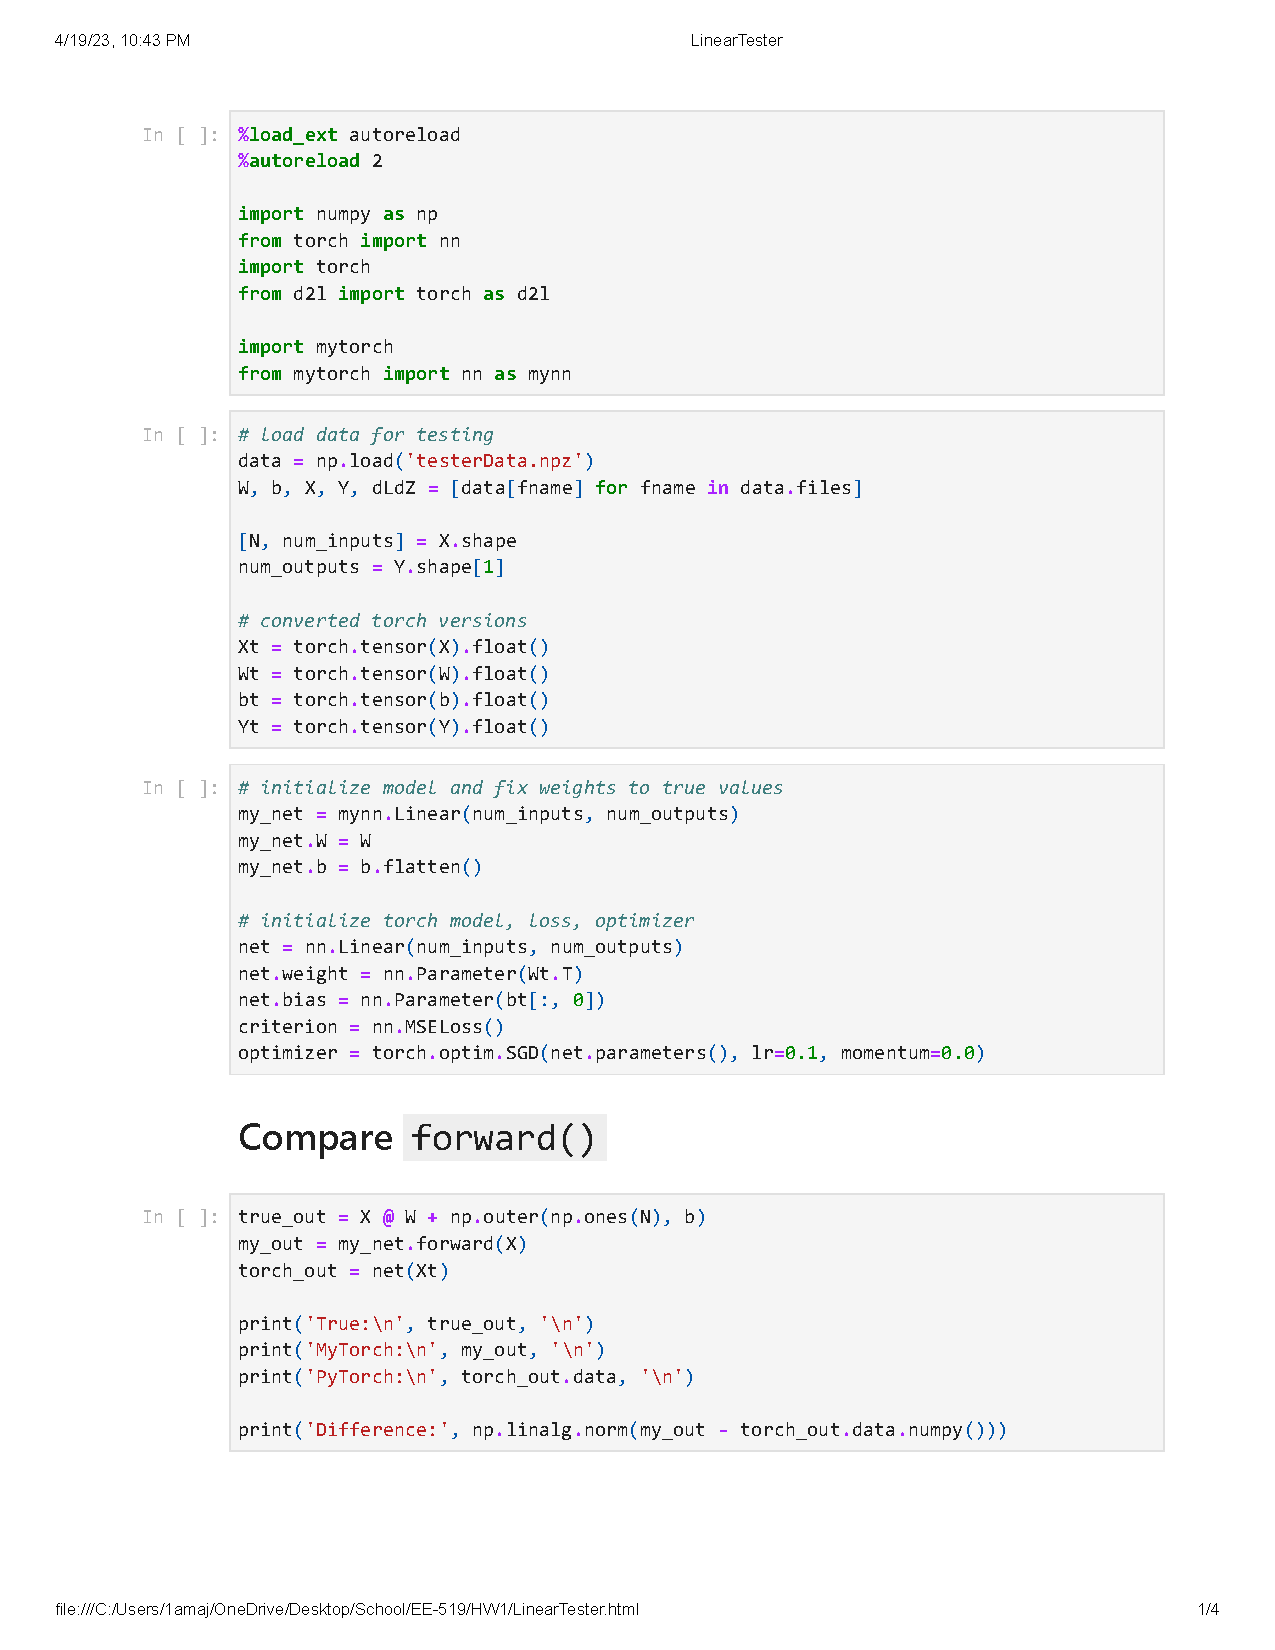
\includepdf[pages=-]{LinearTester.pdf}

\clearpage
\section{\normalfont{\texttt{loss.py} (2 pts each)}}

Your next task is to implement both the mean squared error (MSE) and cross entropy losses as their own classes in \texttt{loss.py}. Defining these classes allows us to treat losses as objects, which allows for storing and passing gradients.

\begin{enumerate}[(a)]
    \item Implement the \texttt{forward} method for the \texttt{MSELoss} class. This method takes as inputs the output matrix $O \in \bR^{N \times q}$ and returns the MSE with respect to the true targets $Y \in \bR^{N \times q}$. Note that the MSE is normalized by dividing by $Nq$ rather than just $N$.
    \item Implement the \texttt{backward} method for the \texttt{MSELoss} class. This method takes no input arguments and uses the stored variables $O$ and $Y$ to compute and return $\dLdO$.
    \item Implement the \texttt{forward} method for the \texttt{CrossEntropyLoss} class. This method takes as inputs the output matrix $O \in \bR^{N \times q}$ and returns the MSE with respect to the true targets $Y \in \bR^{N \times q}$. Note that the cross entropy loss is normalized by dividing by $N$ only.
    \item Implement the \texttt{backward} method for the \texttt{CrossEntropyLoss} class. This method takes no input arguments and uses the stored variables $O$ and $Y$ to compute and return $\dLdO$.
\end{enumerate}
\textbf{Turn in} the output of the notebook \texttt{LossTester.ipynb}.\\

\textbf{Answer:}\\

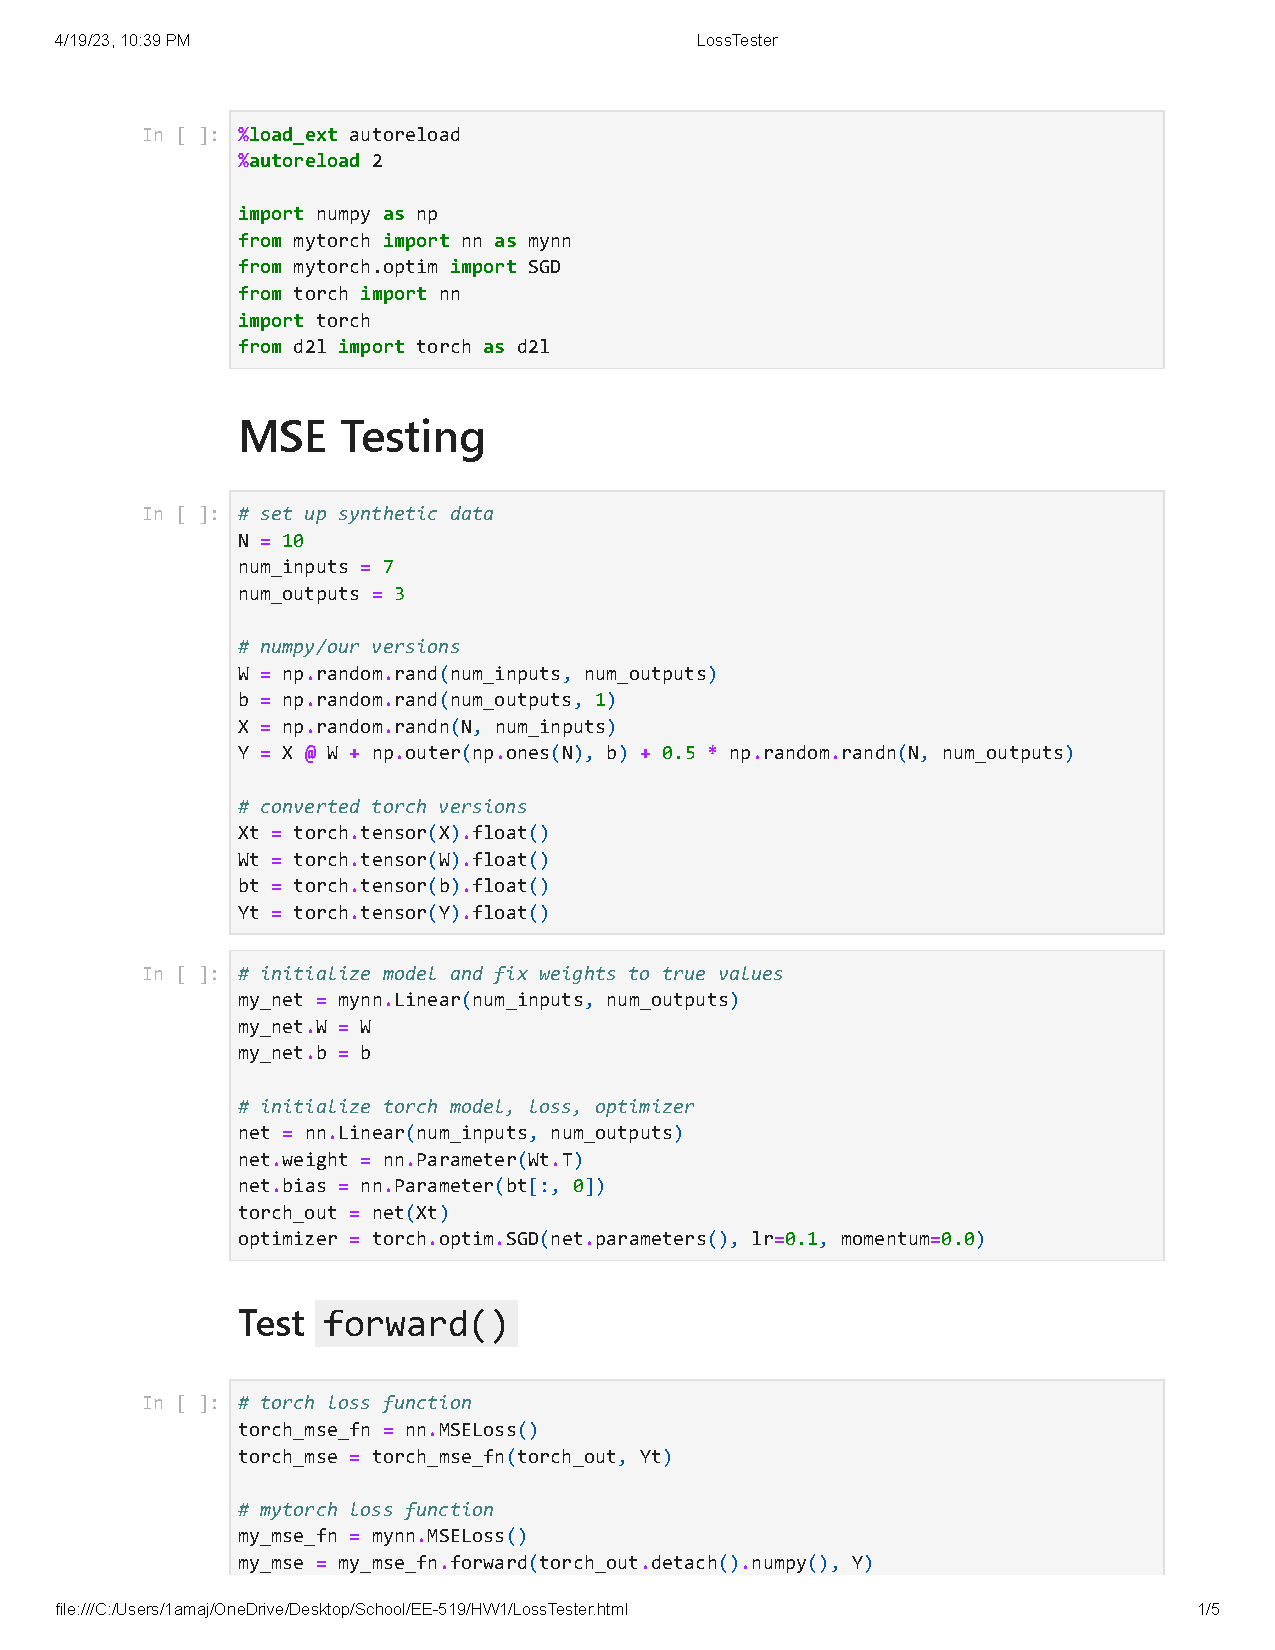
\includepdf[pages=-]{LossTester.pdf}

\clearpage
\section{\normalfont{\texttt{sgd.py} (2 pts)}}

Now that we have the ability to pass gradients, we can use stochastic gradient descent (SGD) to optimize the parameters of our linear layer. Your task is to implement the \texttt{step} method, which updates both the weight matrix $W$ and bias vector $b$. Note that the provided implementation allows for multiple layers, but the update equation is the same for either case.

\noindent \textbf{Turn in} the output of the notebook \texttt{SGDTester.ipynb}.\\

\textbf{Answer:}\\

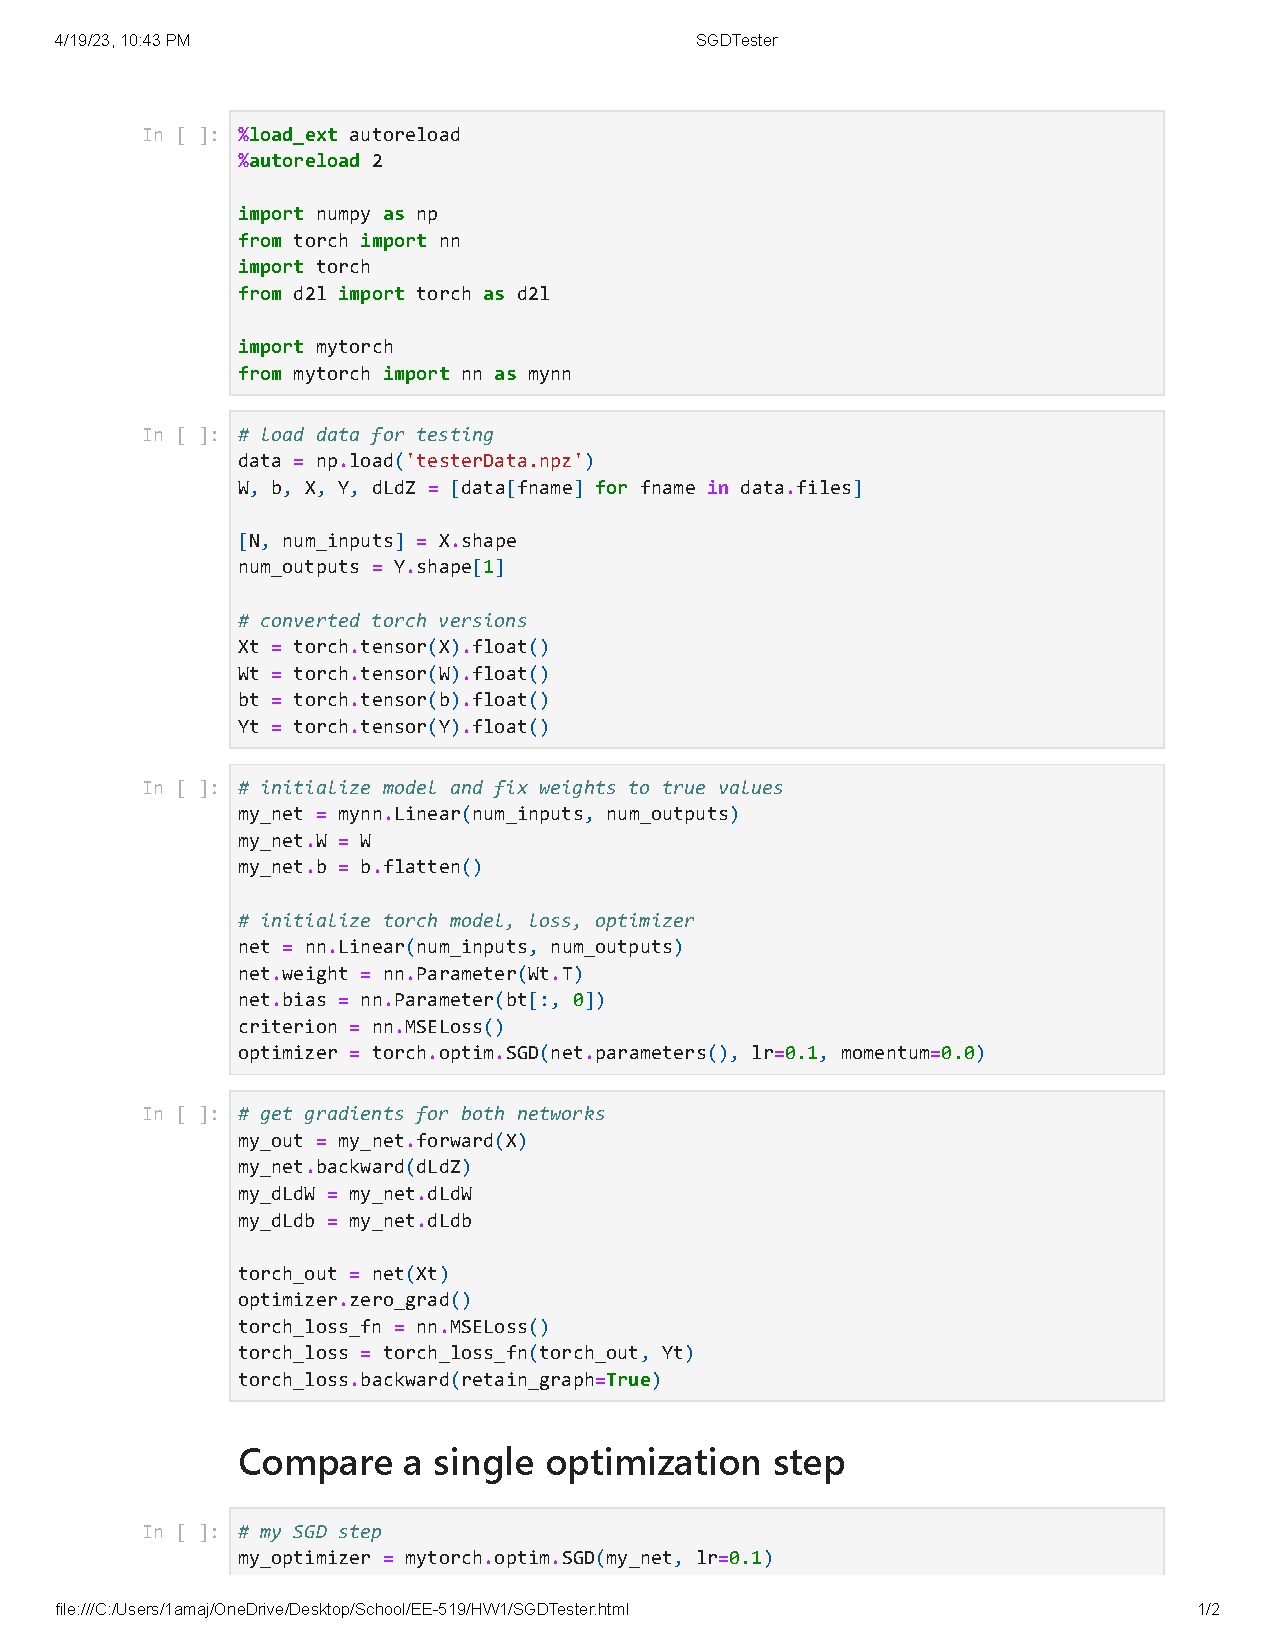
\includepdf[pages=-]{SGDTester.pdf}

\clearpage
\section{\normalfont{\texttt{activation.py} (2 pts each)}}

At this point, we have implemented a single-layer neural network that can be used for either classification or regression. You can (and probably should) test your network using the notebook \texttt{TrainingTester.ipynb} to see how it performs on these tasks. To allow our network to learn nonlinear functions, we need to utilize activation functions, which are implemented in \texttt{activation.py}.

Consider a multi-layer perceptrion (MLP) with a single hidden layer. Let $H \in \bR^{N \times h}$ be the output of hidden variables after the first linear layer. For an activation function $\phi: \bR \to \bR$, let $A \in \bR^{N \times h}$ be the output after applying $\phi$ element-wise to $H$.

\begin{enumerate}[(a)]
    \item Implement the sigmoid activation function. Complete the \texttt{forward} method, which takes the hidden variables $H$ as input and outputs the the activation function applied element-wise to $H$. Next, complete the \texttt{backward} method, which utilizes the stored variable $H$ to compute the element-wise gradient of the activation function with respect to $H$. Note that the gradient $\partial A / \partial H$ should have the same dimensions as $H$.
    \item Implement the $\tanh$ activation function, completing both the \texttt{forward} and \texttt{backward} methods.
    \item Implement the ReLU activation function, completing both the \texttt{forward} and \texttt{backward} methods.
\end{enumerate}
\textbf{Turn in} the output of the notebook \texttt{ActivationTester.ipynb}.\\

\textbf{Answer:}\\

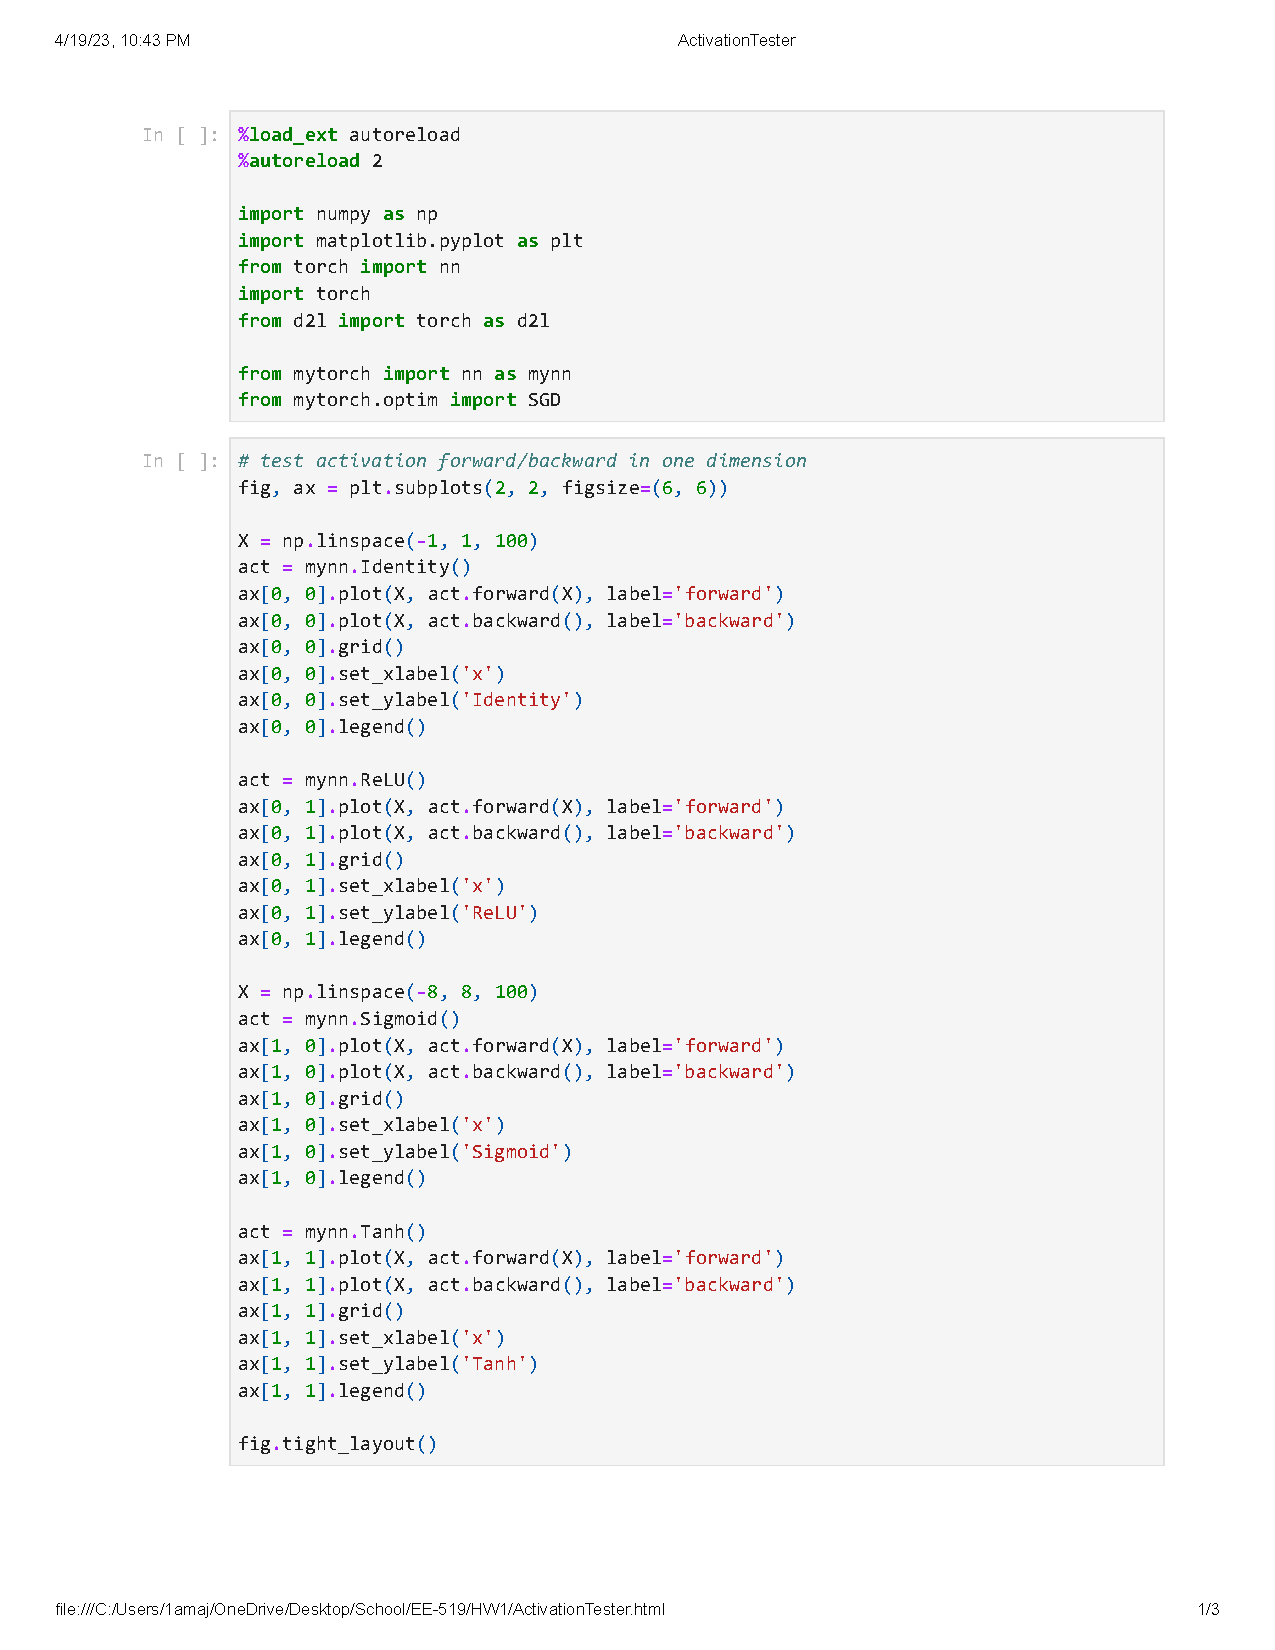
\includepdf[pages=1-]{ActivationTester.pdf}

\clearpage
\section{\normalfont{\texttt{mlp.py} (4 pts each)}}

Having put into place the tools for optimizing a linear layer, selecting the appropriate cost function, and adding nonlinearities, we are now ready to implement a MLP with an arbitrary number of layers. In this problem, we will complete the \texttt{mlp.py} file, implementing MLPs with 0, 1, and 4 hidden layers.

\begin{enumerate}[(a)]
    \item Complete the class \texttt{MLP0} to implement an MLP with 0 hidden layers. The class structure is as follows.
        \begin{itemize}
            \item \texttt{\_\_init\_\_}: Defines the list of layers in \texttt{self.layers} and activation functions in \texttt{self.f}. For the MLP0, we have one linear layer and a single Identity activation function.
            \item \texttt{forward}: Performs a forward pass, first through the linear layer, then through the activation function. The parameters follow the equations
                \begin{align*}
                    H^{(1)} &= X W^{(1)} + 1_{N} (b^{(1)})^{T} \\
                    A^{(1)} &= \phi\left( H^{(1)} \right) \; \text{(element wise)}
                \end{align*}
            \item \texttt{backward}: Performs a backward pass through the network. This method takes the gradient $\partial L / \partial A^{(1)}$ as input, then computes $\partial A^{(1)} / \partial H^{(1)}$ via the \texttt{backward} method for the corresponding activation function. It then computes
                \begin{equation*}
                    \frac{\partial L}{\partial H^{(1)}} = \frac{\partial L}{\partial A^{(1)}} \odot \frac{\partial A^{(1)}}{\partial H^{(1)}}.
                \end{equation*}
                Noting that $H^{(1)}$ is the output of our single linear layer, it uses $\partial L / \partial H^{(1)}$ to compute the gradients of the loss with respect to $W^{(1)}$, $b^{(1)}$, and the inputs $X$. These gradients can be used with SGD or passed to additional layers, as in parts (b) and (c) of this problem.
        \end{itemize}
    \item Complete the class \texttt{MLP1} to implement an MLP with 1 hidden layer. In this case, our forward equations become
        \begin{align*}
            H^{(1)} &= X W^{(1)} + 1_{N} (b^{(1)})^{T} \\
            A^{(1)} &= \phi\left( H^{(1)} \right) \; \text{(element wise)} \\
            H^{(2)} &= A^{(1)} W^{(2)} + 1_{N} (b^{(2)})^{T} \\
            A^{(2)} &= \phi\left( H^{(2)} \right) \; \text{(element wise)}.
        \end{align*}
    \item Follow the above sequence to complete the class \texttt{MLP4}.
\end{enumerate}
\textbf{Turn in} the output of the notebook \texttt{MLPTester.ipynb}.\\

\textbf{Answer:}\\

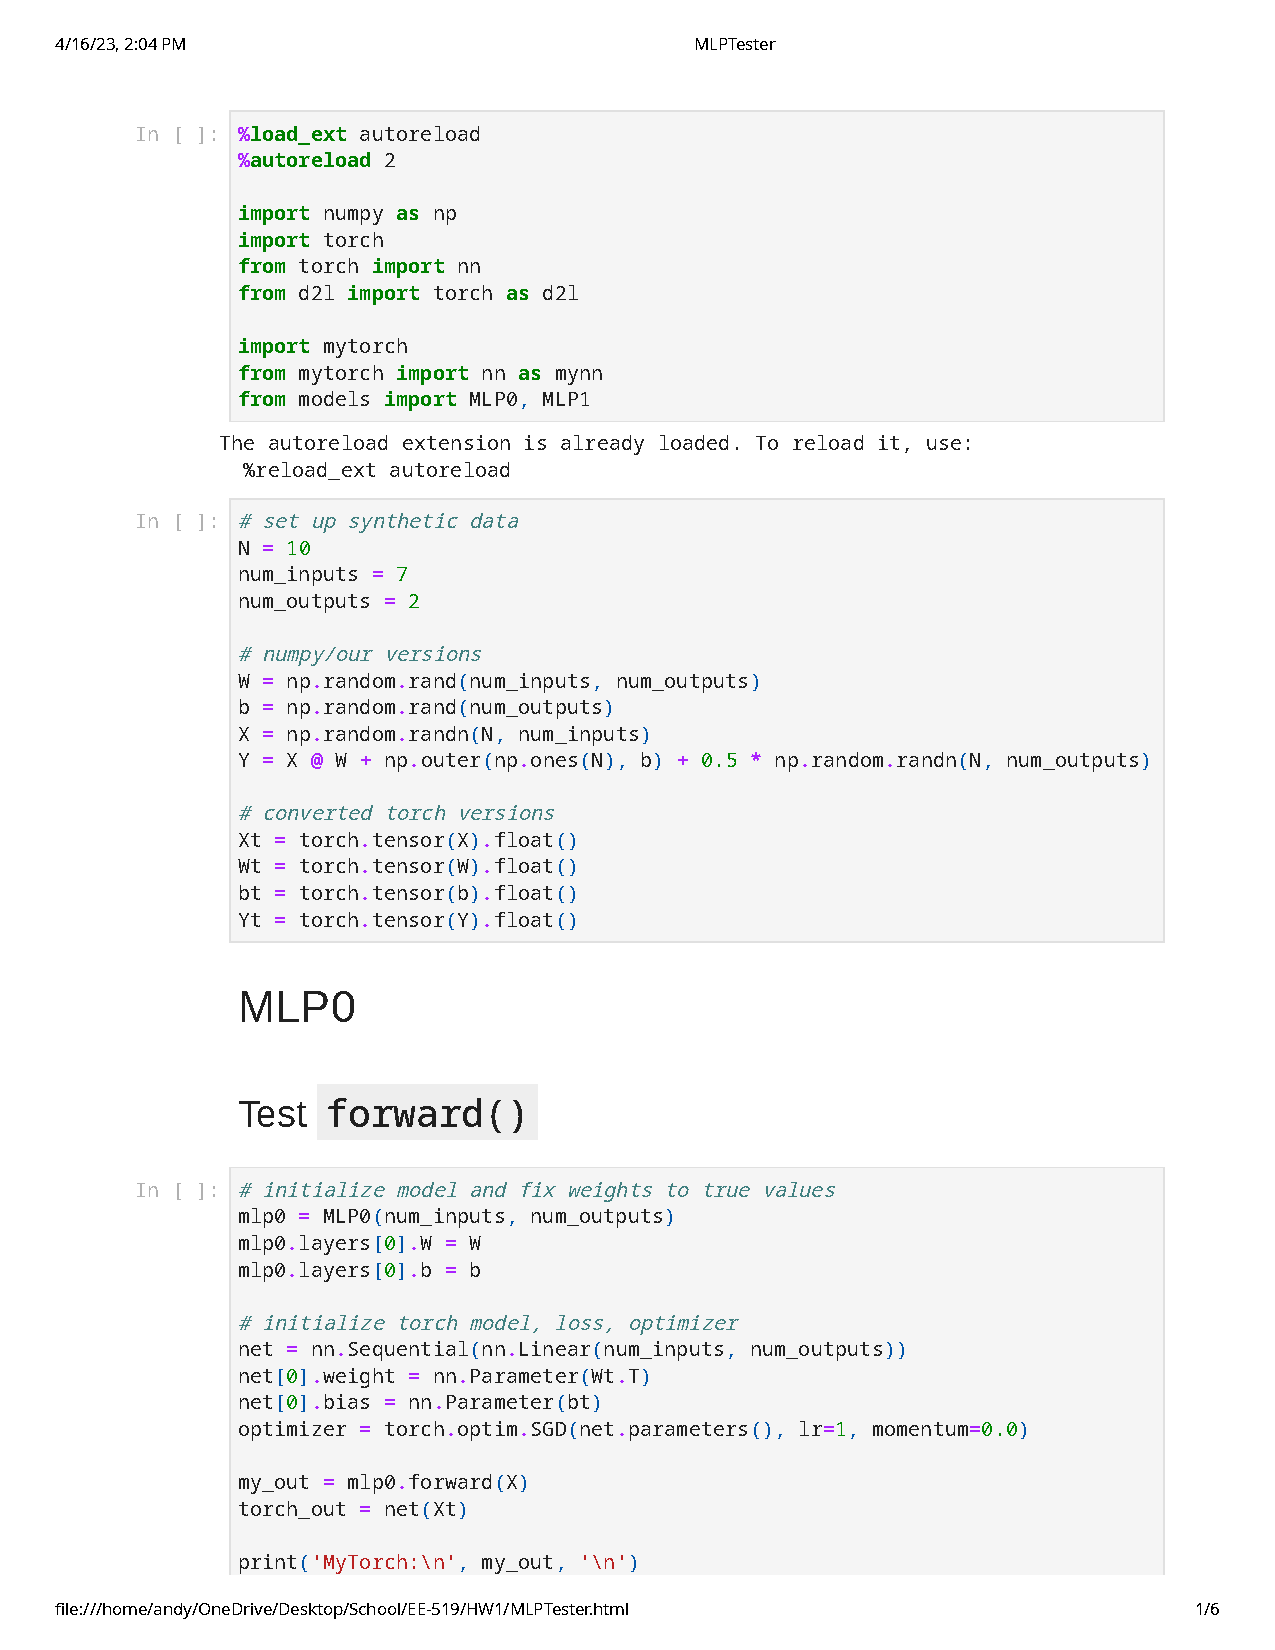
\includepdf[pages=-]{MLPTester.pdf}
\clearpage
\section{\normalfont{\texttt{TrainingTester.ipynb} (0 pts)}}

Congratulations! If you've reached this point, you have coded a pure-\texttt{numpy}, object-oriented implementation of an MLP with arbitrary number of layers and activation functions, capable exciting tasks such as regressing synthetic data and classifying pictures of clothing! In \texttt{TrainingTester.ipynb}, I have implemented the framework to allow for training neural networks with MyTorch using tools from the D2L library. Have a look at the code in this notebook to
observe what changes were required to utilize our library, as well as how to perform the same tasks using PyTorch.

\vspace{1em}
\noindent \textbf{Turn in} nothing.

\textbf{All code:}\\

\textbf{Linear Code:}\\
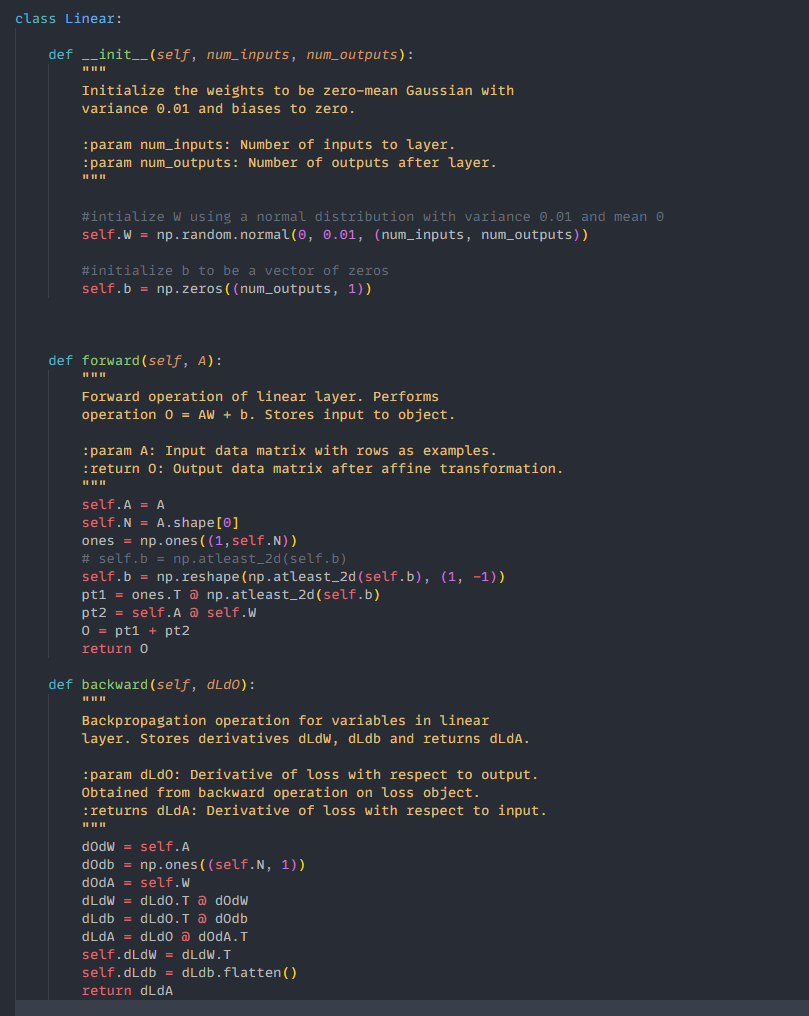
\includegraphics[width=1\textwidth]{LinearCode.png}\\
\textbf{Loss Code:}\\
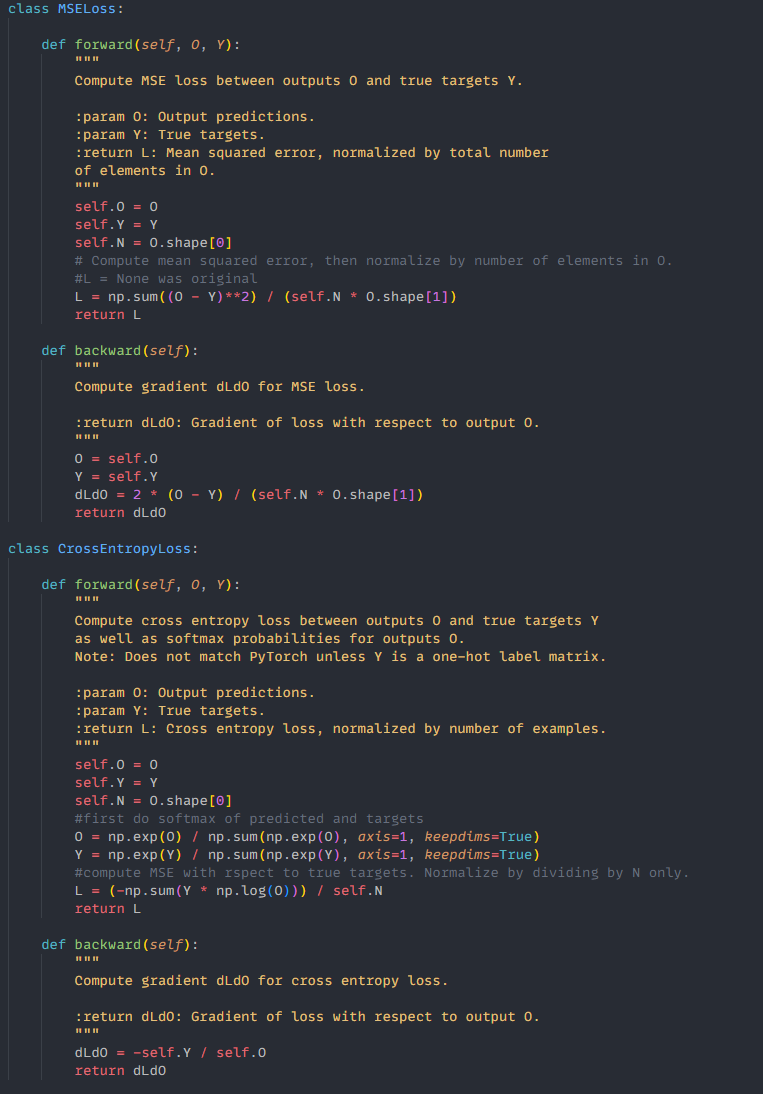
\includegraphics[width=1\textwidth]{LossCode.png}\\
\textbf{SGD Code:}\\
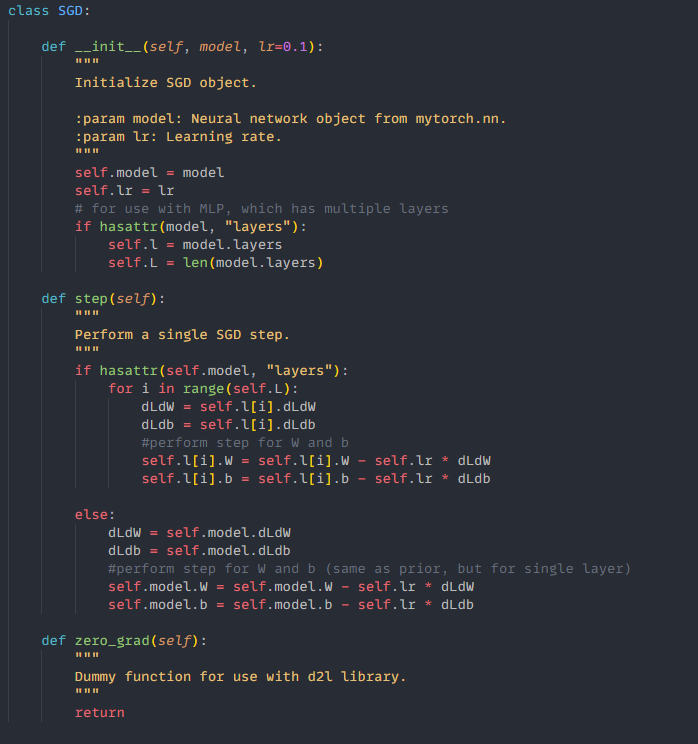
\includegraphics[width=1\textwidth]{SGDCode.png}\\
\textbf{Activation Code:}\\
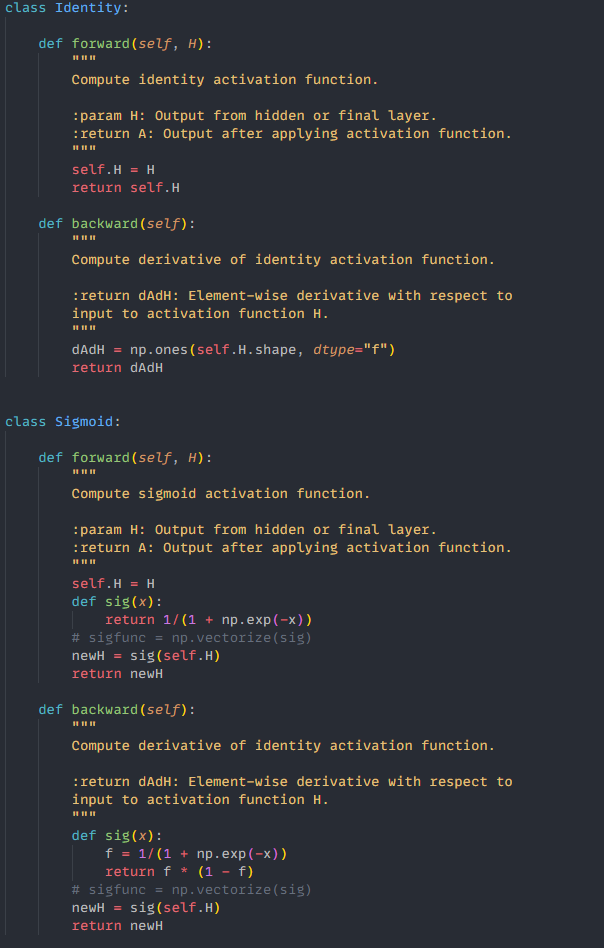
\includegraphics[width=0.5\textwidth]{ActivationCode1.png}
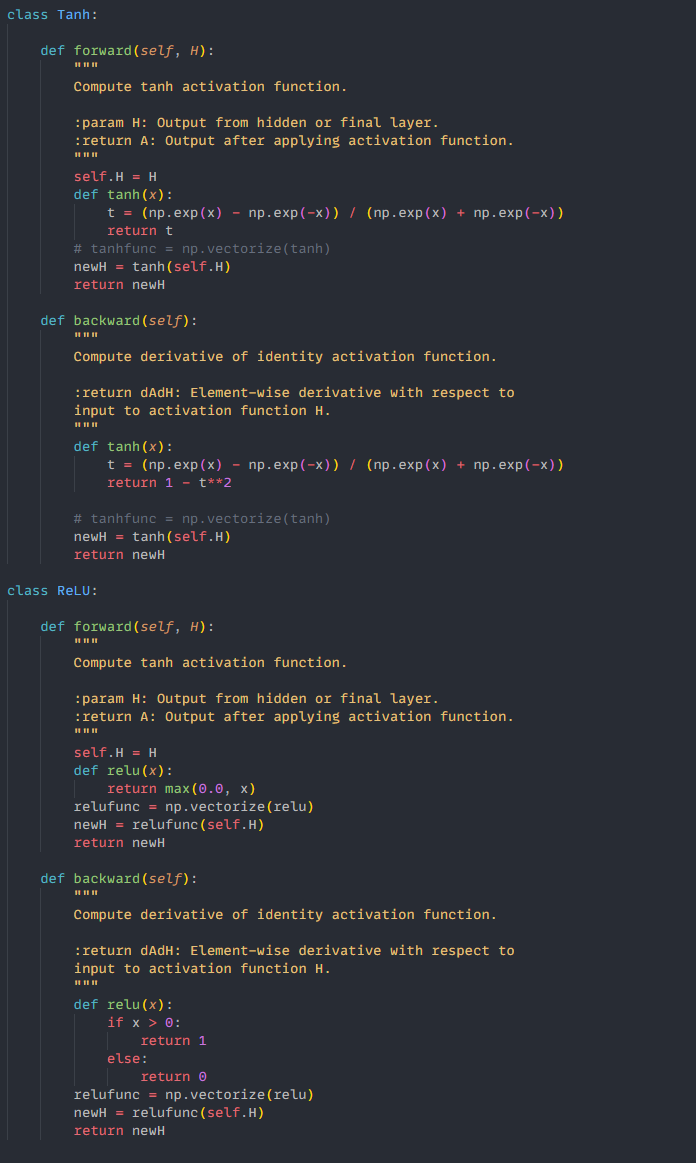
\includegraphics[width=0.5\textwidth]{ActivationCode2.png}\\

\textbf{MLP Code:}\\
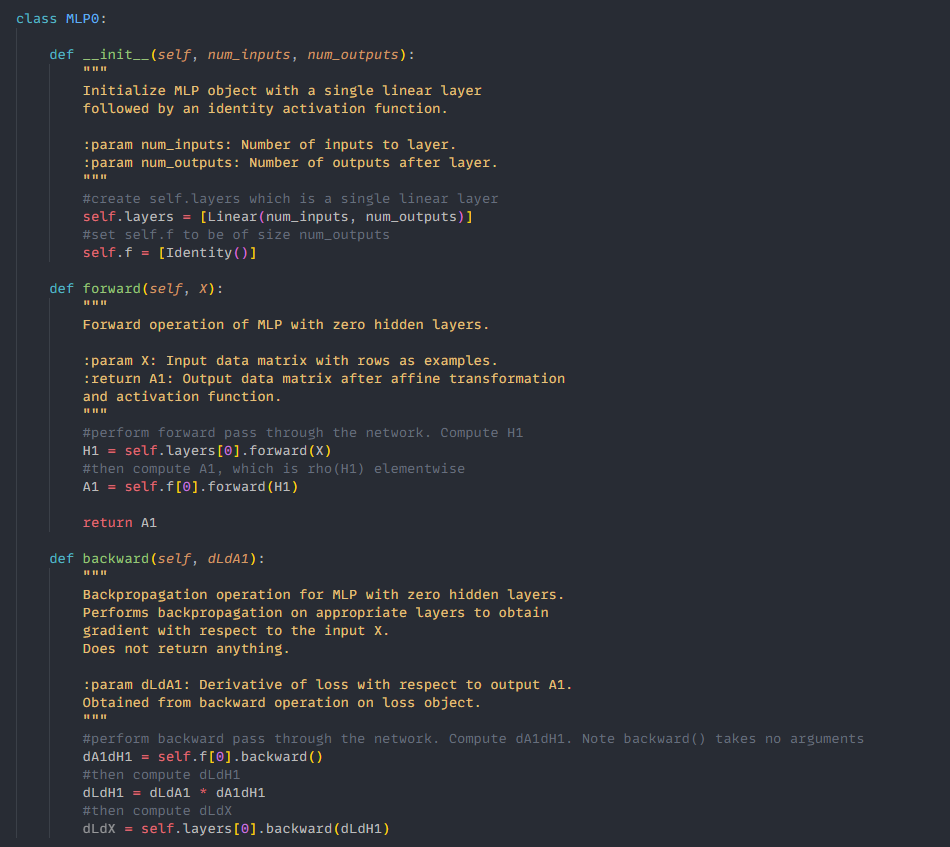
\includegraphics[width=1\textwidth]{MLP0.png}
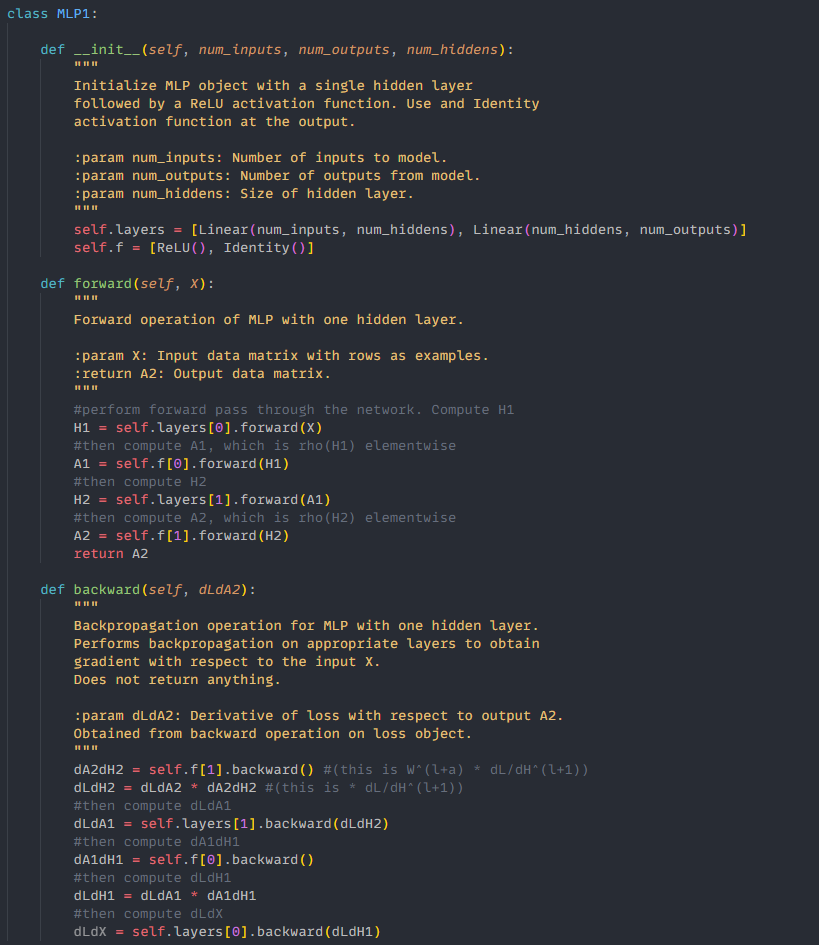
\includegraphics[width=1\textwidth]{MLP1.png}
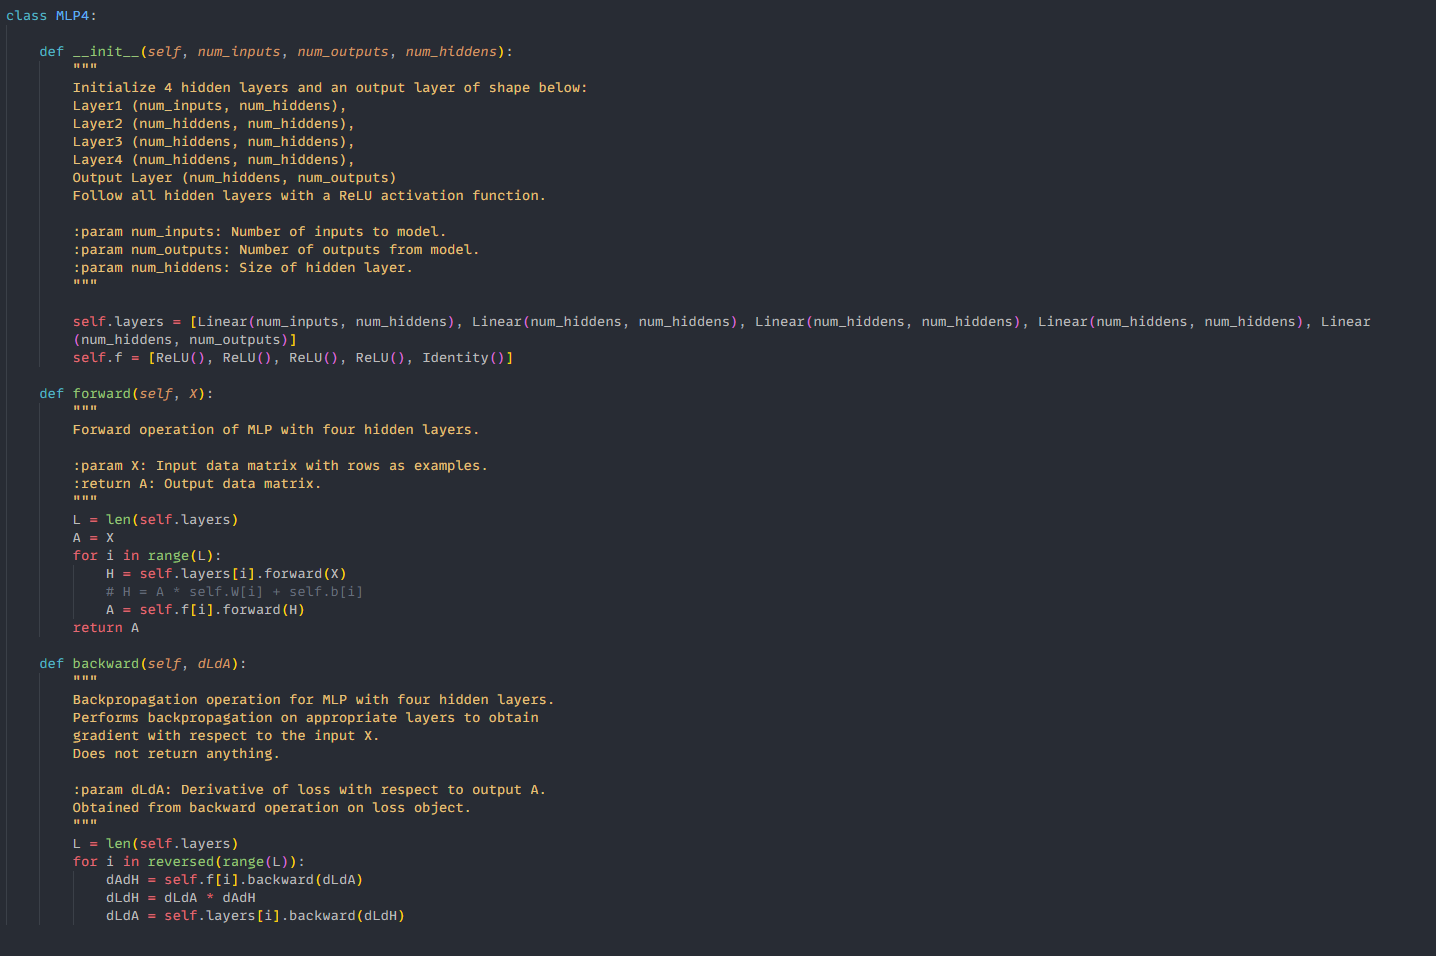
\includegraphics[width=1\textwidth]{MLP2.png}
\end{document}
